\chapter{Background}
\label{sec:background}

\section{General Feature Extraction Algorithms}
\label{sec:genFeatureExtract}
This chapter describes two feature extraction algorithms, 2D SURF and BRISK, on which the algorithms used for this thesis are based. From here on in, \textit{Detector} will refer to the module of the feature extraction algorithm that is used to detect the interest points. \textit{Descriptor} will refer to the module of the feature extraction algorithm that computes the descriptor for each interest point.\\


\subsection{2D SURF}
\label{sec:2dsurf}
The SURF feature extraction algorithm is based on approximating the Hessian matrix at every point in an image. The determinant of the Hessian is then computed at each point and is referred to as the blob response. This computation is performed over a number of different scales in scale space as well as in image space in order to find local maxima. A non-maximal suppression is then performed and the local maxima that exist after this stage will be defined as interest points. Each interest point is represented by a descriptor of length $64$. Interest points in different images are then matched based on the Euclidean distance between their respective feature vectors. The smaller the distance, the more certain the match becomes. 

\subsubsection{Integral Images}
\label{sec:integralImages}
One of the big advantages in SURF over SIFT \citep{Lowe2004} is its computational efficiency. One of the important tools that are utilised in order to create this advantage in computation is called the Integral Image \citep{Bay2008}. An integral image computes the integral image value $I_{int}(x,y)$ for pixel location $(x,y)$  as a sum of all pixel intensities found to the left and below the current pixel location until the origin. This is presented in \eqnref{eqn:integralImage}. The variable $I(x,y)$ is the individual pixel intensity at location $(x,y)$. Thus the value of each pixel can be interpreted as the area of the rectangle formed from the current pixel to the image origin. It is assumed that the image origin is in the top left corner of the image. \\

\begin{equation}
I_{int}(x,y) = \sum_{i=0}^{i \leq x}\sum_{j=0}^{j \leq y}I(x,y)
\label{eqn:integralImage}
\end{equation}

By computing the integral image, it is possible to reduce the calculation of any upright rectangular image to four operations. This is very useful when computing box filter convolutions that will be described in the sections to follow.\\

\subsubsection{Detector}
\label{2dsurfdetect}
The SURF detector is based on computing the determinant of the Hessian matrix. The Hessian matrix is a matrix of second order partial derivatives and, when calculated for an intensity image   $I(x,y)$, it is of the form shown in \eqnref{eqn:hessian}.\\

\begin{equation}
Hessian = \left[ \begin{array}{cc} \frac{\partial I}{\partial x^2} & \frac{\partial I}{\partial x^2}\\
					    \frac{\partial I}{\partial x^2} & \frac{\partial I}{\partial x^2}\end{array} \right]
\label{eqn:hessian}
\end{equation}

The Hessian matrix is computed in order to identify local maxima and minima in the image. This is achieved by first computing the determinant, also know as the discriminant, of the Hessian matrix. The determinant of the Hessian is shown in \eqnref{eqn:determinant}. If the determinant of the Hessian is negative then a local extremum has not been identified. If the determinant is positive then a local extremum has been identified \citep{Evans2009}. \\

\begin{equation}
det\mid H \mid = \frac{\partial I}{\partial x^2} \frac{\partial I}{\partial y^2} - (\frac{\partial I}{\partial x \partial y})^2
\label{eqn:determinant}
\end{equation}

For a SURF detector, the Hessian is computed for a point $\textbf{x} = (x,y)$ in the Image $I$. The Hessian is computed over multiple scales, $\sigma$, and therefore the Hessian matrix at a point for a specific scale is represented as $H(\textbf{x}, \sigma)$ \citep{Lowe2004} and is defined as shown in \eqnref{eqn:hessianScale}.\\


\begin{equation}
H(\textbf{x}, \sigma) = \left[ \begin{array}{cc} L_{xx}(\textbf{x}, \sigma) & L_{xy}(\textbf{x}, \sigma)\\
					    L_{xy}(\textbf{x}, \sigma) & L_{yy}(\textbf{x}, \sigma)\end{array} \right]
\label{eqn:hessianScale}
\end{equation}

The variable $L_{xx}(\textbf{x}, \sigma)$ is analogous to the second order derivative, $ \frac{\partial I}{\partial x^2}$, detailed in \eqnref{eqn:hessian}. This second order derivative is computed in SURF detectors by convolving the image, at point $\textbf{x}$, with a particular kernel \citep{Evans2009}. The kernel in this instance is the second order Gaussian derivative, $\frac{\partial g(\sigma)}{\partial x^2)}$. \\

There are a number of reasons why Gaussians are used as the kernel in computing the second order derivatives. One of the main reasons is that it is possible to vary the amount of smoothing resulting from the convolution of the Gaussian with the image \citep{Evans2009}. This enables the calculation of the Hessian determinant at different scales which is used for non-maximal suppression and identifying scale-invariant interest points.\\

The SURF implementation approximates Gaussian second order derivatives for the convolution stage by using box filters. Box filters are used to perform very fast convolutions. A box filter consists of positive and negative lobes. Each lobe is assigned a particular weighting. For example, in \figref{fig:boxFilters} \citep{Bay2008}, the white lobes are assigned a weighting of positive one, the black lobes are assigned a weighting of negative one and the gray lobes are assigned a weighting of zero. The box filters are created in the $x$, $y$ and $xy$ directions in order to compute the Hessian and subsequently its determinant. One of the key advantages to this approach is the computational cost. This is because it is possible to use a combination of integral images and box filters to perform the second order derivative computation very efficiently. It is also possible to increase the size of the box filters at no additional computational cost \citep{Bay2008}.\\

\begin{figure}[h!] 
  \centering
    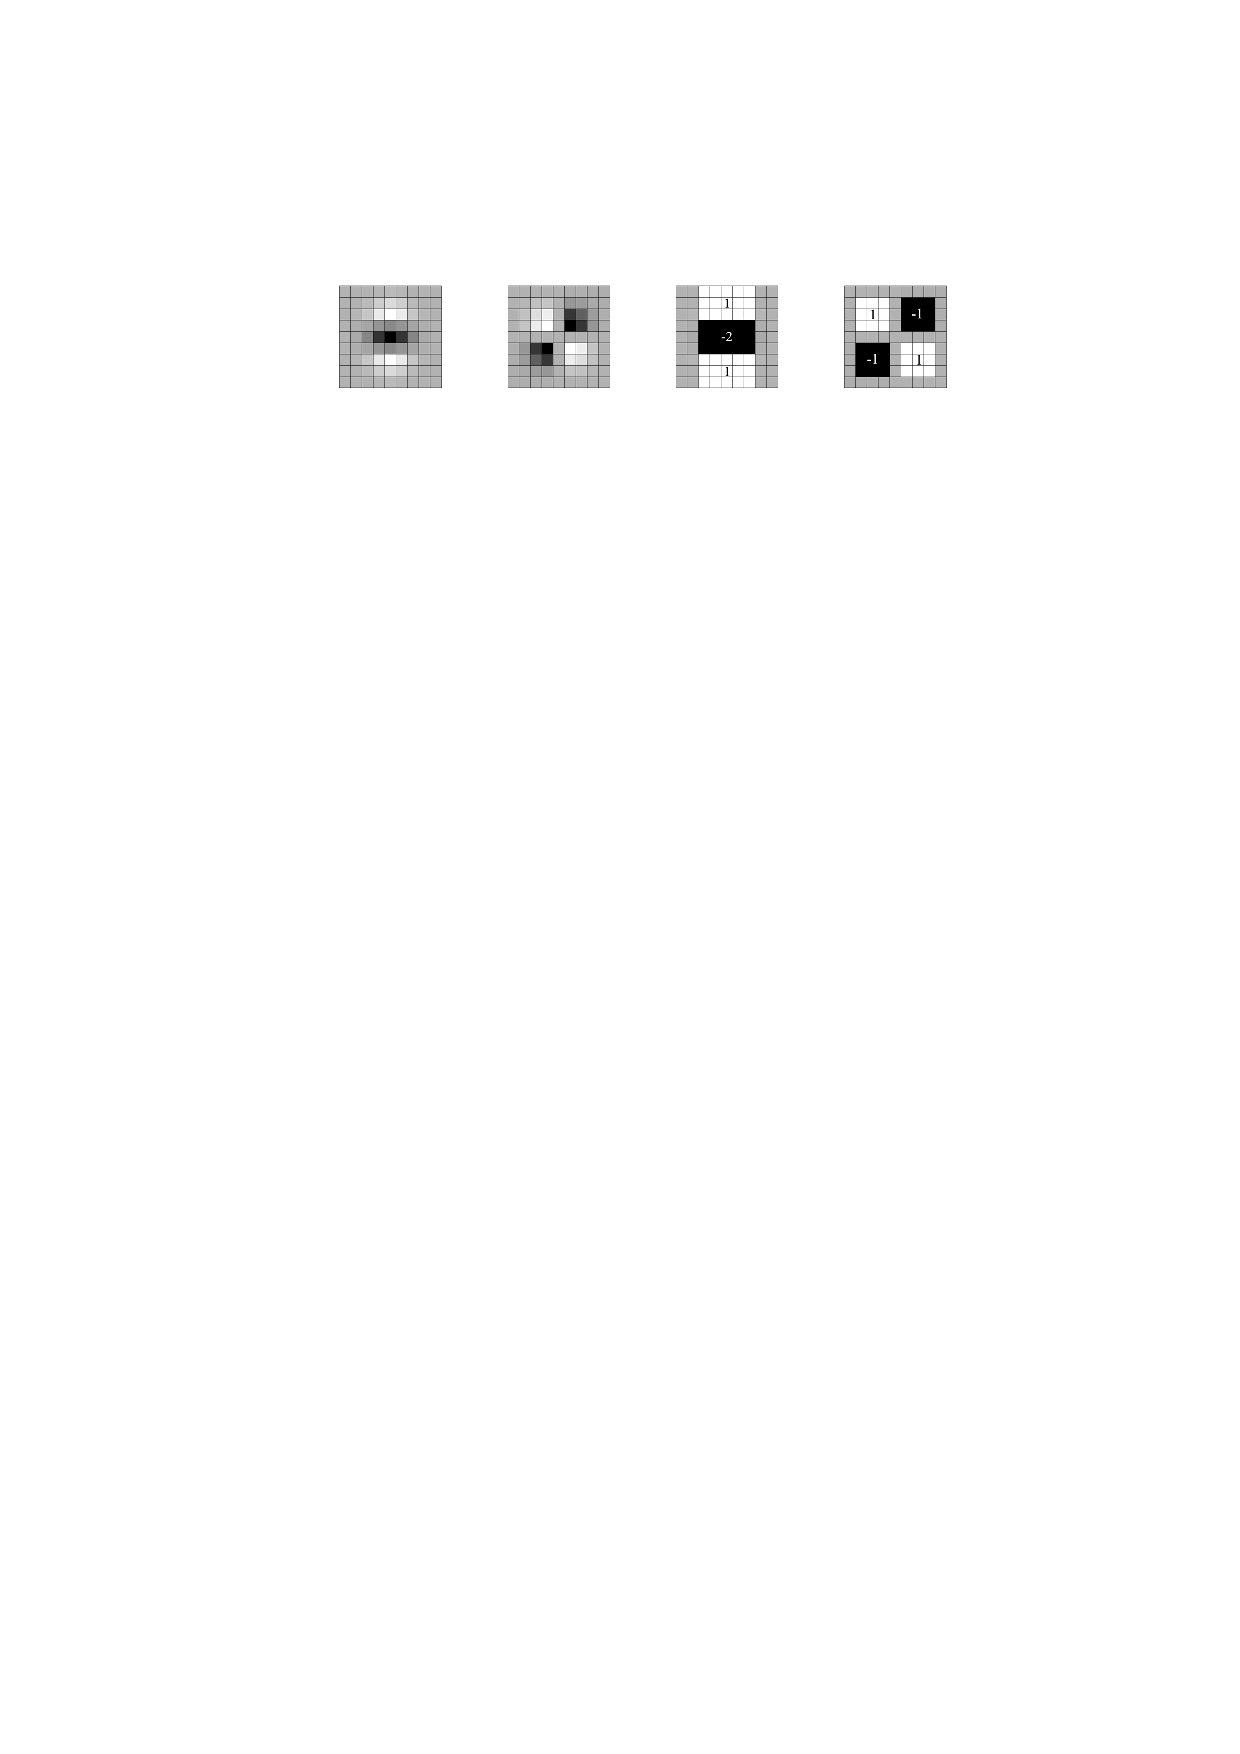
\includegraphics[width=0.8\textwidth]{../Drawings/methods/SURF2D_BoxFilters.pdf}
    \caption{The Box filters used to perform the 2D convolutions}
    \label{fig:boxFilters}
\end{figure}

Therefore, utilising box filters, the determinant of the Hessian is computed as shown in \eqnref{eqn:approxHessian}. The variables $D_{xx}$, $D_{xy}$ and $D_{yy}$ represent the box filter convolutions in the $x$, $xy$ and $y$ directions respectively at a point $\textbf{x} = (x,y)$ in the image $I$.\\ 

\begin{equation}
det \mid H_{approx} (x,y) \mid = D_{xx}D_{yy} - (0.9 D_{xy}^2)
\label{eqn:approxHessian}
\end{equation}

The determinant of the Hessian at a point $\textbf{x} = (x,y)$ in the image $I$ is referred to as the blob response at a scale $\sigma$ \citep{Bay2008}. The blob response is computed at every location in the image in order to create a blob response map. A blob response map exists for every considered scale and these maps are used to detect local maxima in the images.\\

The different scales collectively define the scale space. The scale space can be seen as a function that is used to find extrema across a set of predefined scales. A set of scales is important as interest points need to be found across a number of scales in order to verify that the point is indeed an interest point. It also ensures that the point can be detected at different scales (I.e. points of view).\\

In the SIFT method \citep{Lowe2004}, in order to construct the scale space, an image is convolved with a Gaussian kernel. The image is then sub-sampled and re-convolved with the same kernel to create a new scale. In the SURF method, as mentioned previously, the box filter size can be increased at no computational cost due to the use of integral images. Thus it makes sense to construct the scale space by convolving the image with the box filters, but instead of sub-sampling the image, the box filters can be increased in size and convolved with the same image at very little computational cost. This creates a very efficient `inverted' scale space pyramid as shown in \figref{fig:scaleSpace} \citep{Evans2009}. The higher the position in the pyramid, the larger the scale and vice versa. \\

\begin{figure}[h!] 
  \centering
    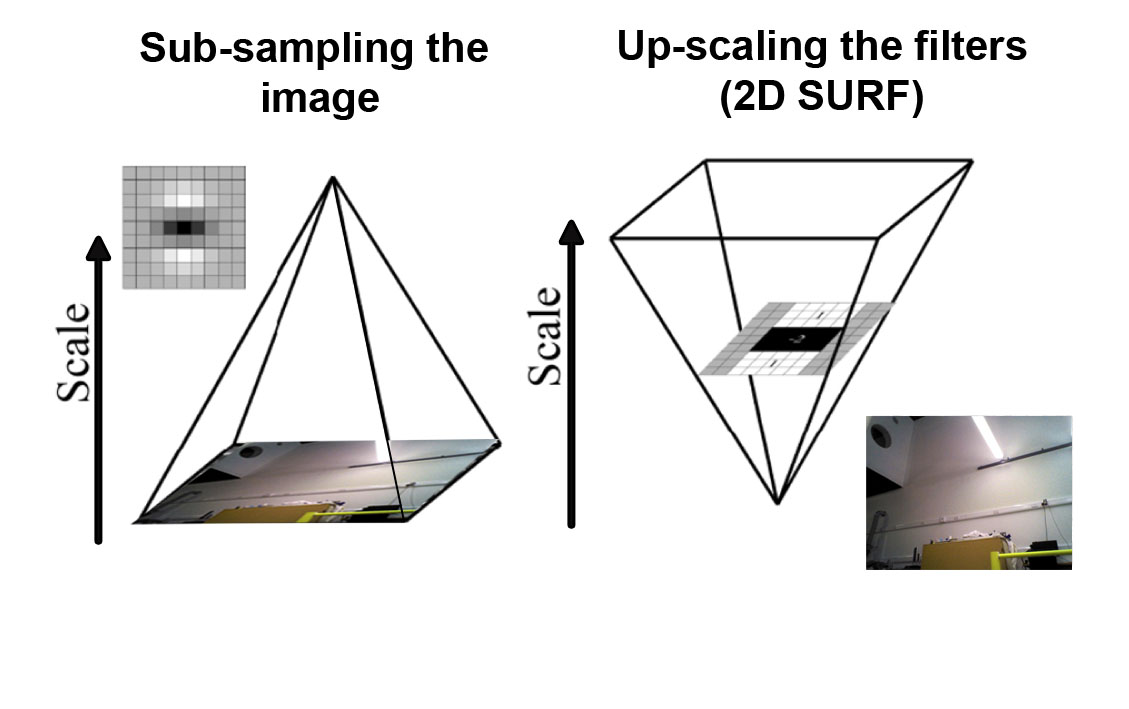
\includegraphics[width=0.8\textwidth]{../Drawings/methods/SURF2D_Image_pyramid.jpg}
    \caption{The up-scaling of the filters is used in 2D SURF rather than the down-scaling of the image}
    \label{fig:scaleSpace}
\end{figure}

The scale space is divided into octaves. An octave consists of a set of blob response maps each resulting from a convolution of the image with a box filter of a specific size. The blob response map corresponding to the lowest level (i.e. smallest scale) of the scale space is constructed using a $9 \times 9$ box filter. This corresponds to a scale value of $1.2$. As the size of the filters used for convolution increase, so too does the scale. During the convolution procedure, the filter is centered on each $(x,y)$ location in the image and each lobe in the filter has a specific width represented by $l_0$. In order to increase the size of the filter (I.e. move up a level in scale space), the filter lobe width, $l_0$, is increased by $2$ pixels. This ensures that the center pixel is still found in the center of the filter. Thus, the first filter is $9 \times 9$ and the next successive filter is $15 \times 15$. \\

The number of octaves used to find interest points depends on the size of the image. Usually, three to four octaves are used. The first octave uses box filters of size $9 \times 9$, $15 \times 15$, $21 \times 21$ and $27 \times 27$ to convolve with the current image.  For each subsequent octave, the filter size increase is doubled. Therefore, for example, the second octave will have filter sizes of $15 \times 15$, $27 \times 27$, $39 \times 39$ and $51 \times 51$ respectively. This corresponds to a filter increase of $12$ pixels. The next octave will have an increase of $24$ pixels and so on \citep{Bay2008}. \\

As mentioned previously, the convolution of the box filters of various sizes produces blob response maps at various scales. The next step involves using the blob response maps to detect interest points at these different scales. The first step in detecting interest points is removing pixels whose blob responses are below a certain threshold. Once the relevant pixels have been thresholded,  a non-maximal suppression is performed in a $3 \times 3 \times 3$ neighborhood surrounding the current pixel. Thus for each octave and each scale within the octave, each pixel is compared to its $26$ neighbors \citep{Evans2009}. This includes its $8$ adjacent neighbors in image space as well as its $9$ neighbors in the scale above and scale below the current image space respectively as shown in \figref{fig:imageSpace} \citep{Lowe2004}. It should be noted that the largest scale and smallest scale for each octave have no scale space layers above or below respectively. Therefore these blob response maps are only used for comparison for the internal scale space layers. \\

\begin{figure}[h!] 
  \centering
    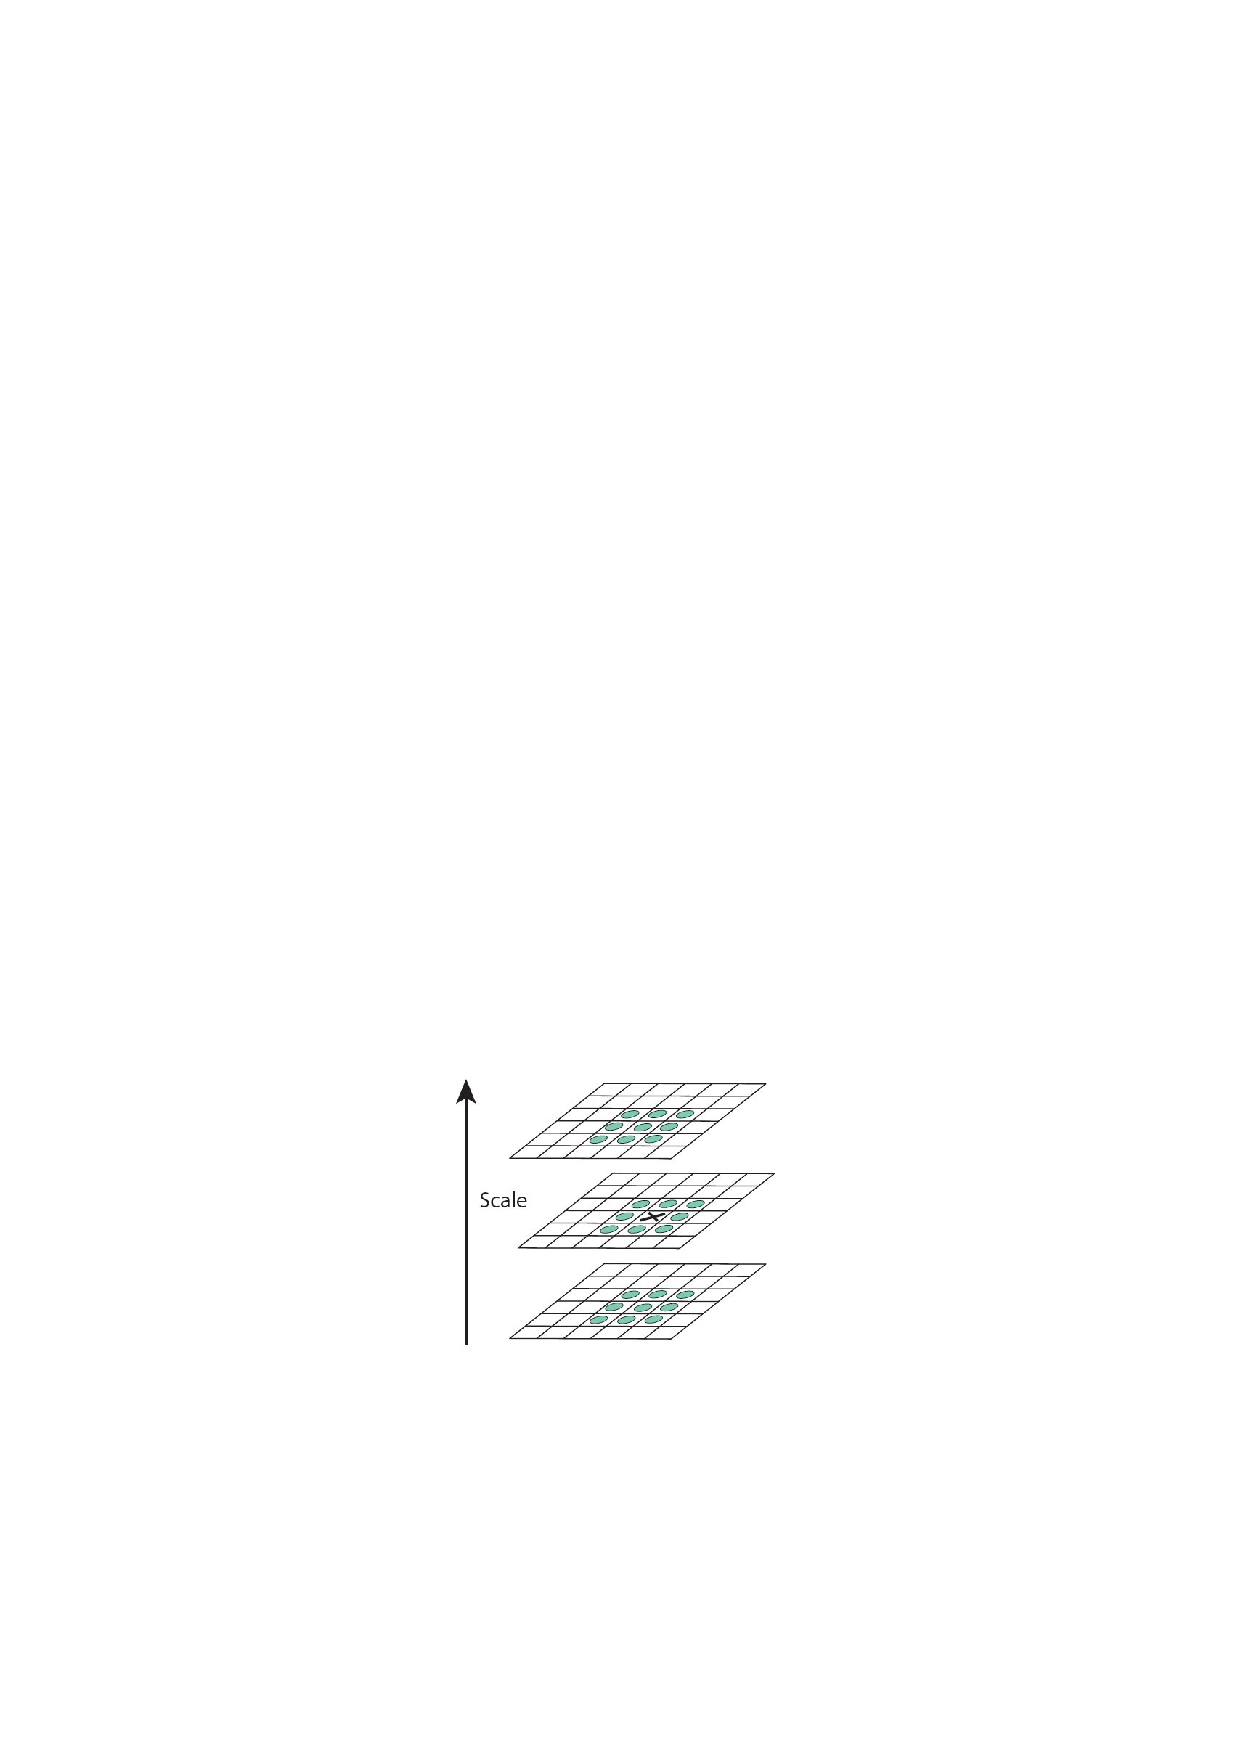
\includegraphics[width=0.5\textwidth]{../Drawings/methods/SURF2D_Nonmaximal_suppression.pdf}
    \caption{The non-maximal suppression performed on each point and its $26$ surrounding neighbors}
    \label{fig:imageSpace}
\end{figure}

If the pixel is not suppressed, then its image space and scale space locations are calculated to sub-pixel accuracy using a linear interpolation procedure \citep{Evans2009}. The pixel becomes an interest point and its descriptor then needs to be determined.\\

%The interpolation procedure TO DO Maybe...

\subsubsection{Descriptor}
\label{sec:2dsurfdescribe}
The SURF descriptor is a $64$ length vector that contains information about the intensity content of the neighborhood surrounding the interest point. In developing the descriptor, a number of important steps need to be implemented. The first step is creating a reproducable orientation for the interest point \citep{Bay2008}. If the interest point is detected at a scale, $\sigma$, then Haar Wavelets of size $4\sigma$ are used to calculate Haar Wavelet Responses (HWRs) for all pixels within a circular radius of $6\sigma$ from the detected interest point.  Haar Wavelets are simple filters that are used in SURF to calculate gradients in the $x$ and $y$ directions respectively. Examples of these wavelets are shown in \figref{fig:haar} \citep{Evans2009}. Once the HWRs have been calculated, they are then weighted by a Gaussian whose mean is centered on the interest point. This means that the pixels found further away from the interest point have a smaller influence on the reproducible interest point orientation.\\


\begin{figure}[h!] 
  \centering
    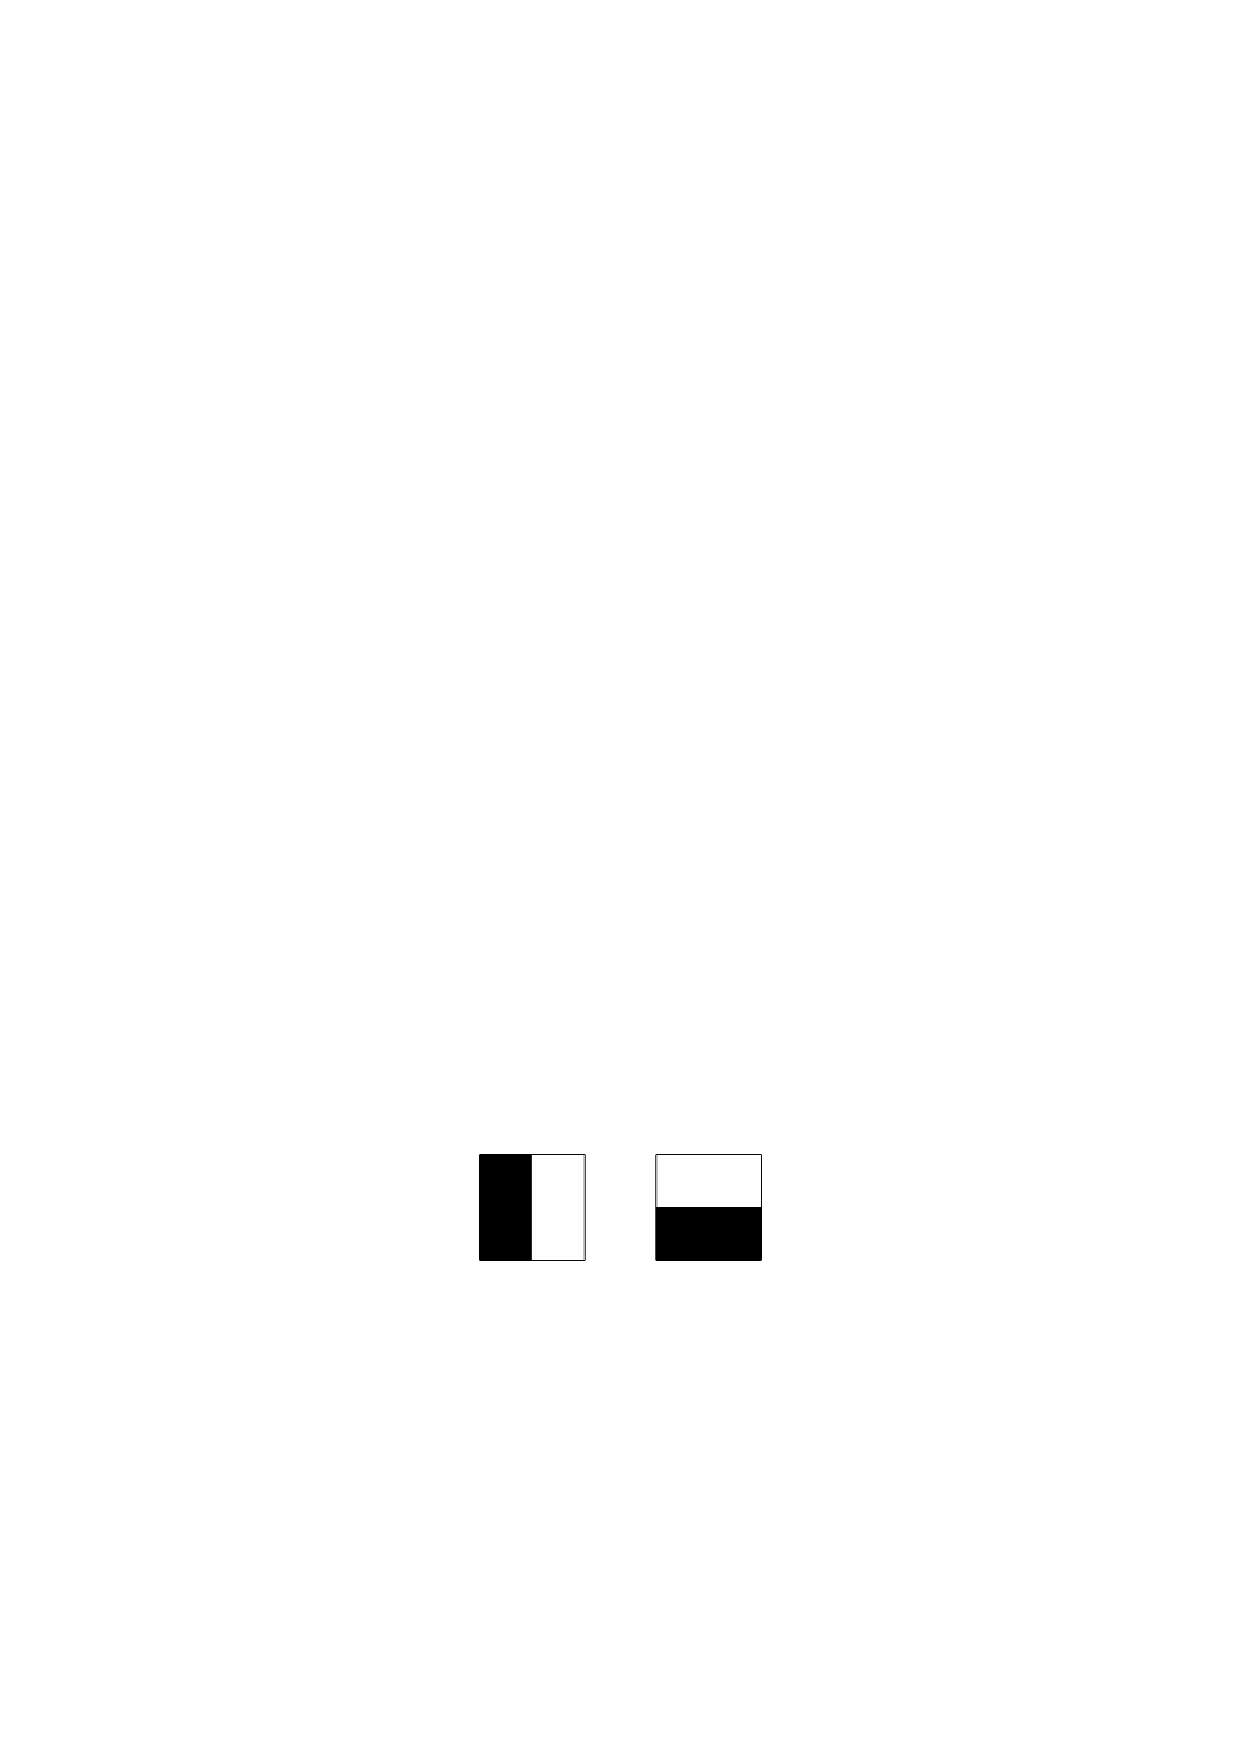
\includegraphics[width=0.5\textwidth]{../Drawings/methods/SURF2D_HaarWavelets.pdf}
    \caption{Haar Wavelets used to calculate the Haar Wavelet Responses. The left Haar Wavelet calculates the responses in the $x$ direction and the right one calculates the Haar Wavelets in the $y$ direction}
    \label{fig:haar}
\end{figure}

In order to find the reproducible orientation, a circular segment of width $\frac{\pi}{3}$ is rotated around the interest point and the HWRs in the $x$ and $y$ directions, within this circular segment, are calculated to yield a vector for that particular circular segment as shown in \figref{fig:circularSegment} \citep{Evans2009}. The longest vector resulting from the rotation of this circular segment around the interest point is assigned to the interest point as the reproducible orientation.\\

\begin{figure}[h!] 
  \centering
    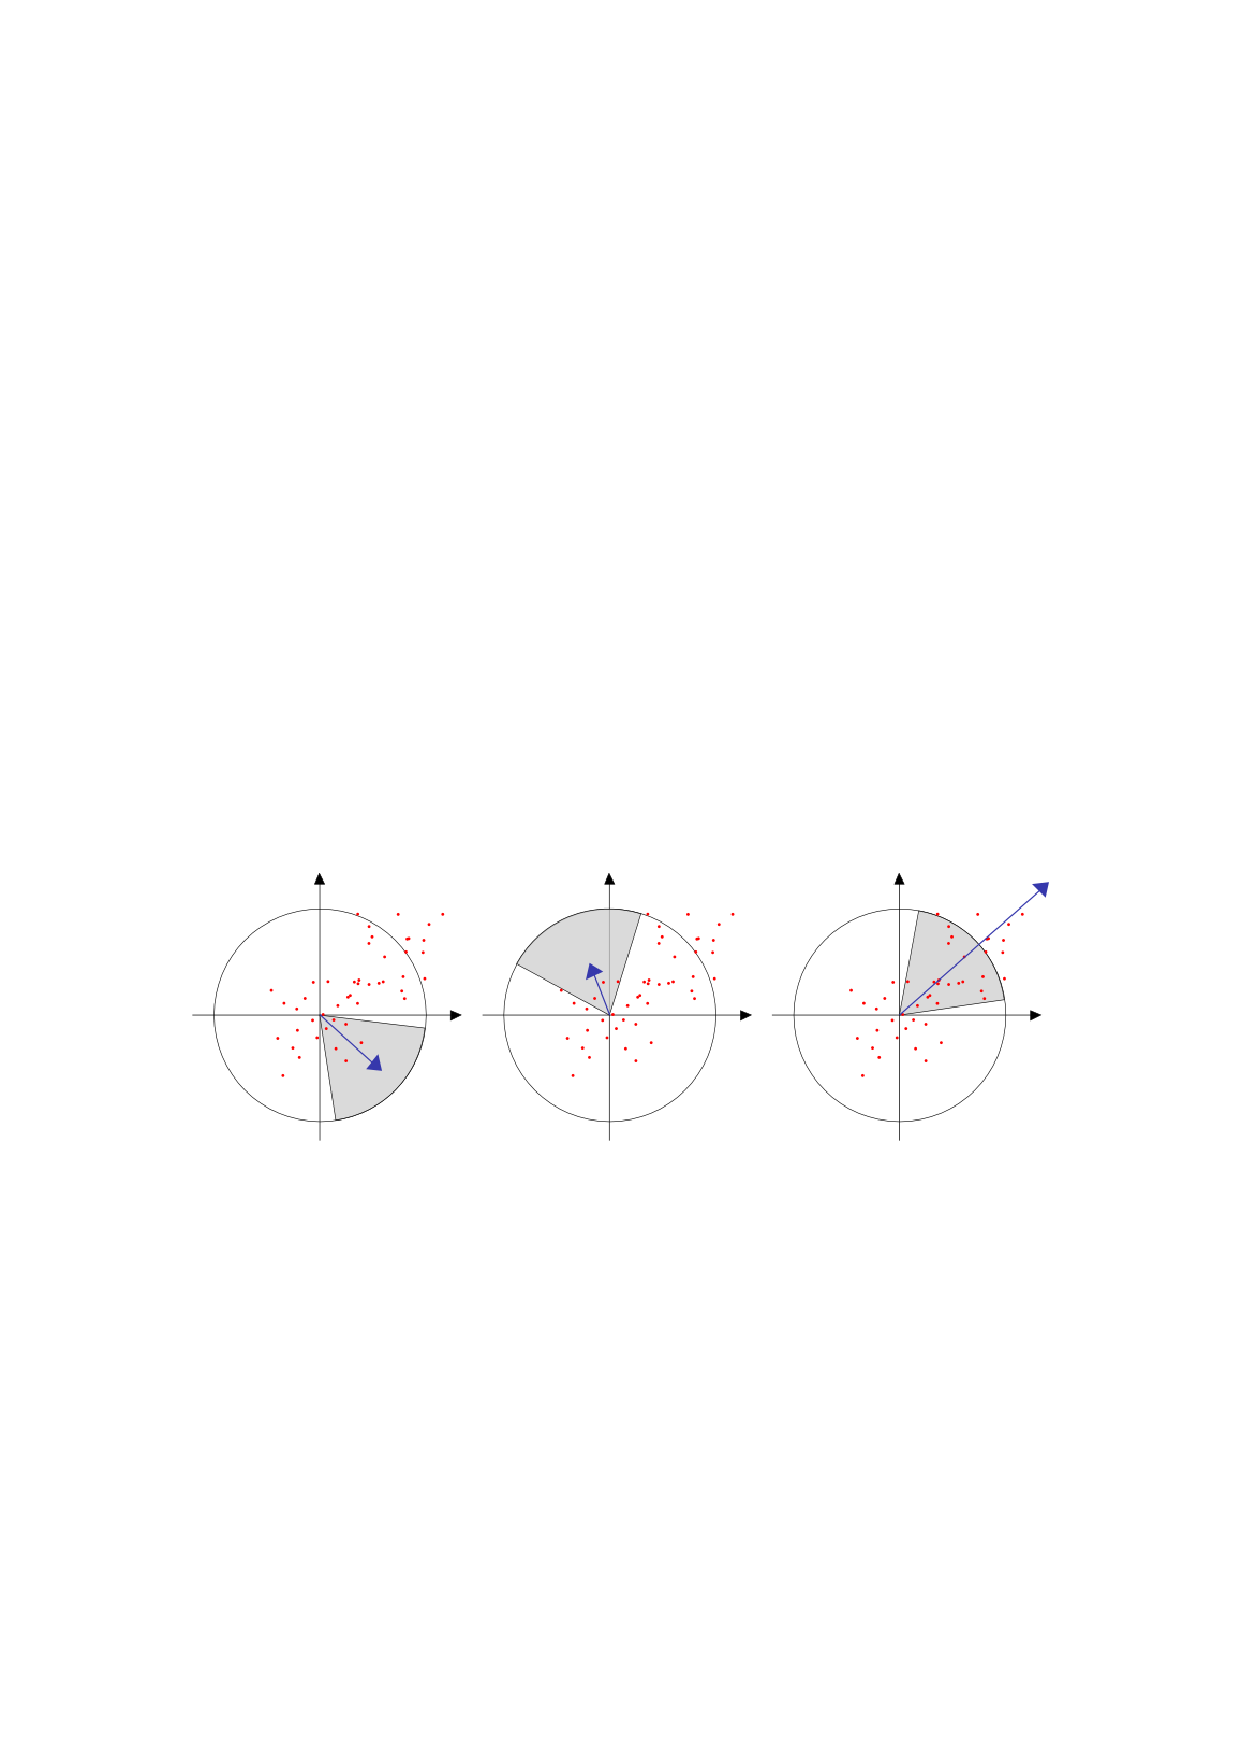
\includegraphics[width=1.0\textwidth]{../Drawings/methods/SURF2D_orientation_assignment.pdf}
    \caption{The $\frac{\pi}{3}$ circular segment calculating the Haar Wavelet Responses for a particular interest point. Here, the right-most figure contains the largest vector and the interest point is therefore assigned the orientation of this vector}
    \label{fig:circularSegment}
\end{figure}

Once the orientation of the interest point has been determined, a square window of size $20\sigma$ is centered around the interest point and is oriented in the direction of the reproducible orientation of that interest point. This square region is then split into $16$ sub-regions of equal size. In each sub-region, HWRs in the $x$ and $y$ directions are then computed for $5 \times 5$ regularly spaced sample points. It is important to note that the $x$ and $y$ directions are relative to the reproducible orientation axes as shown in \figref{fig:reproducibleAxes} \citep{Evans2009}. The HWRs for these $25$ sample points are then summed together to yield the descriptor for the sub-region as shown in \eqnref{eqn:descriptorSub}. Since there are $16$ of these sub-regions, a $64$ length descriptor is created.\\

\begin{figure}[h!] 
  \centering
    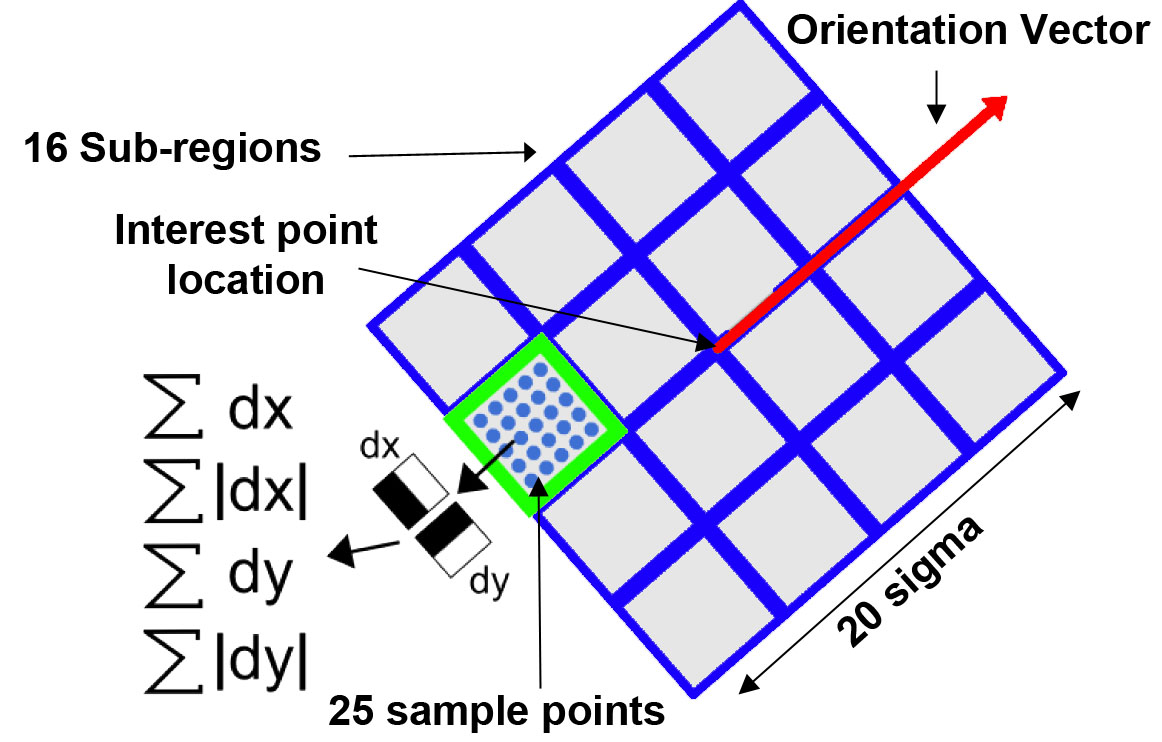
\includegraphics[width=0.5\textwidth]{../Drawings/methods/SURF2D_Descriptor.jpg}
    \caption{The square window centered on the interest point and aligned with the orientation vector}
    \label{fig:reproducibleAxes}
\end{figure}

\begin{equation}
descriptor_{sub} = [\Sigma d_x, \Sigma d_y,  \Sigma \mid d_x \mid , \Sigma \mid d_y \mid] 
\label{eqn:descriptorSub}
\end{equation} 



\subsection{BRISK}
\label{sec:brisk}
A new method has been developed that, in a variety of domains yields performance that betters SURF by an order of magnitude. This method is called Binary Robust Invariant Scalable Keypoints (BRISK) \citep{Leutenegger2011}. This method utilises a technique called Adapative and Generic Corner Detection Based on the Accelerated Segment Test (AGAST) in order to compute a score for a pixel in location $(x,y)$ in image $I$ \citep{Mair2010}. AGAST is largely based on the Features from Accelerated Segment Test (FAST) \citep{Rosten2006} method but incorporates some improvements such as adaptive tree switching which will be briefly discussed. Using this score, interest points are defined. A binary feature descriptor of length $512$ is then generated for each interest point as a result of some simple brightness comparison tests. Interest points are then matched in different images by computing the Hamming distance between the feature descriptors. \\

\subsubsection{FAST Score}
\label{sec:fastScore}

The FAST score, denoted as $s$, is the first criterion that is used in BRISK in order to identify interest points \citep{Rosten2006}. The FAST score is computed by initially choosing a set of $16$ pixels that form a circle centered on the current pixel $p$. $p$ is the potential interest point that is being evaluated, as shown in \figref{fig:fastScore} \citep{Rosten2006}. The circle has a Bresenham radius of $3.4$ pixels \citep{Mair2010}. In order for the pixel $p$ to be considered an interest point, there has to be a set of $n$ (in this case $9$) contiguous pixels from the circle of $16$ pixels that are brighter than the current pixel intensity, $I_p$, plus some threshold $t$, or are darker than $I_p - t$. A larger value of $t$ will reduce the amount of interest points that will be detected. However, these detected points will be strong, salient interest points. \\

\begin{figure}[h!] 
  \centering
    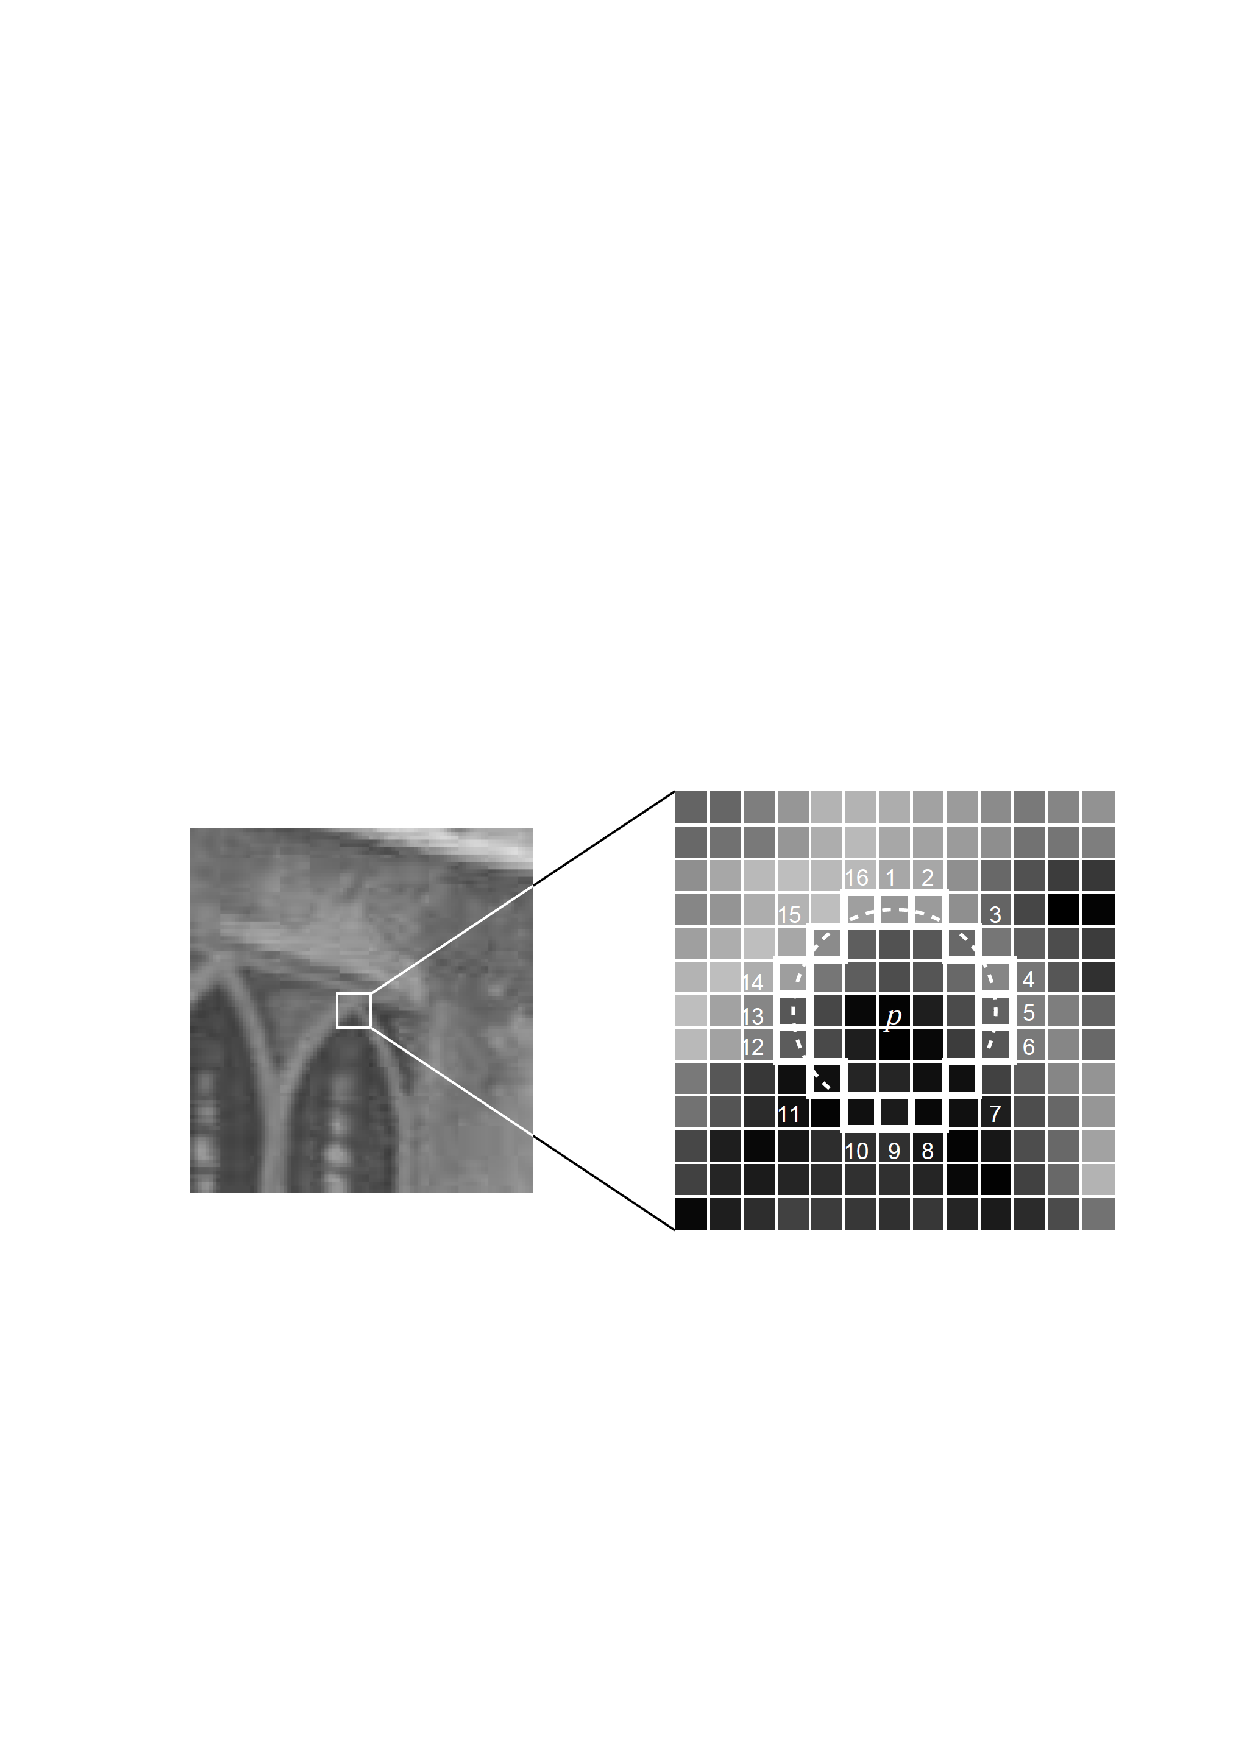
\includegraphics[width=0.8\textwidth]{../Drawings/methods/FASTScoreCalculation.pdf}
    \caption{The calculation of the FAST score for BRISK}
    \label{fig:fastScore}
\end{figure}

The FAST score is computed as the sum of the absolute difference between the circle of pixels and the central pixel. More formally it is expressed as shown in \eqnref{eqn:fastScore}. The variable $I_p$ is the intensity of the central pixel $p$. $I_{p \rightarrow x}$ is the intensity of the pixel at location $x$ on the circle of pixels relative to $p$. $S_{dark}$ refers to all the pixels that are darker than $I_p - t$, whereas $S_{bright}$ refers to all the pixels on the circle that are brighter than $I_p + t$. Taking the maximum of these two quantities yields the FAST score that is used for comparison in determining whether or not the pixel $p$ is an interest point.\\

\begin{equation}
V = max(\sum_{x \epsilon S_{bright}} \mid I_{p \rightarrow x} - I_p \mid - t, \sum_{x \epsilon S_{dark}} \mid I_p - I_{p \rightarrow x} \mid - t)
\label{eqn:fastScore}
\end{equation}

It is important to consider the order in which the points on the circle surrounding the potential interest point are evaluated, for computational efficiency. One method is to evaluate pixels $1, 5, 9 $ and $13$ corresponding to the compass directions \citep{Rosten2006}. At least three of these pixels need to be brighter or darker than the central pixel $p$ plus the chosen threshold in order for the central pixel to be evaluated further. If this is not the case, then the pixel $p$ is discarded as it cannot have $9$ contiguous pixels as mentioned previously and is therefore not an interest point. If at least three of the above-mentioned pixels fulfil the criteria, then the Accelerated Segment Test (AST) is applied to the circle of pixels in order to determine whether or not the central pixel is indeed an interest point. There are different ways of applying the AST in order to determine whether or not a point is an interest point. Both FAST and AGAST use decision trees to search the circle of pixels in a specific order so as to maximise the efficiency with which each potential interest point is evaluated. The techniques differ in terms of the order in which the $16$ circle pixels are evaluated. In addition, AGAST has an adaptive tree switching technique which enables the method to switch to different decision trees that are optimised for a particular area of an image. This has an effect on computational efficiency and how well the methods generalise to different domains.   \\

%FAST performs the AST by first learning a \textit{ternary} tree which has possible pixel states of \textit{brighter}, \textit{darker} or \textit{similar}. In building the tree, at each step, all remaining pixels are asked the question whether or not they are \textit{brighter} or \textit{darker} than the central pixel. The pixel with the highest information gain is chosen as the next branch in the tree. Each pixel can have one of four possible states, namely unknown (u), darker(d), brighter(b) or similar(s). Since $16$ pixels are being evaluated in the circle surrounding the central pixel and each of these pixels have four possible states, there are a total of $4^{16}$ possible configurations. \\
%
%AGAST performs a more efficient and generic AST than that of FAST. One improvement in AGAST's method is that it has a richer configuration space. In addition, a \textit{binary} tree is constructed rather than a \textit{ternary} tree. \textbf{TO DO}\\

\subsubsection{Detector}
\label{briskDetect}
BRISK's scale space has a different structure to that of SURF. In this case, the scale space consists of \textit{n} octaves \textit{$c_i$} and \textit{n} intra-octaves \textit{$d_i$} \citep{Leutenegger2011}. The typical number of octaves chosen for BRISK is $n=4$. The intra-octaves are placed between the octaves. A typical ordering would be $c_0, d_0, c_1, d_1, c_2...$. In order to create the octaves, the image is progressively half-sampled by a factor of two. The first octave corresponding to the original image is called $c_0$ and the first intra-octave $d_0$ is generated by down-sampling the original image by a factor of $1.5$. Thereafter, the image is half-sampled by a factor of two. This creates an image pyramid where the lowest layer is the original image and the higher layers are down-sampled versions of the original image.\\

In BRISK, the FAST score $s$ is computed for each pixel $p$, for each octave and intra-octave respectively \citep{Leutenegger2011}. The same threshold $t$ is used throughout. A non-maximal suppression is then performed on each pixel in every octave and intra-octave respectively. In order to determine whether or not the pixel is indeed an interest point, the pixel $p$ firstly needs to be a maxima (in terms of its FAST score) compared to its $8$ adjacent neighbors in image space. The pixel's FAST score is then compared to the layer above and layer below in the image pyramid. Its FAST score has to be a maxima relative to these values as well. In the case of the original image $c_0$, no layer below this layer exists. To account for this problem, only the layer above $c_0$ is compared.\\

Once a pixel with a maximum score has been detected, a sub-pixel refinement is applied to the maximum by fitting a 2D quadratic function in the least squares sense to a $3 \times 3$ score patch surrounding the detected maximum \citep{Leutenegger2011}. A sub-pixel refinement is also applied to $3 \times 3$ patches in the layers directly above and below the detected maximum in order to generate three local maxima. This procedure is followed by a continuous scale refinement in order to determine the true scale of the detected interest point. A 1D parabola is fitted to these three local maxima along the scale axis as shown in \figref{fig:1dparabola} \citep{Leutenegger2011} and the maximum of this parabola determines the true score and scale of the detected corner. Once the scale has been found, the image coordinates need to be re-interpolated to account for the true scale as the scale may not necessarily lie directly on an octave or intra-octave respectively. This creates a scale invariant interest point.\\

\begin{figure}[h!] 
  \centering
    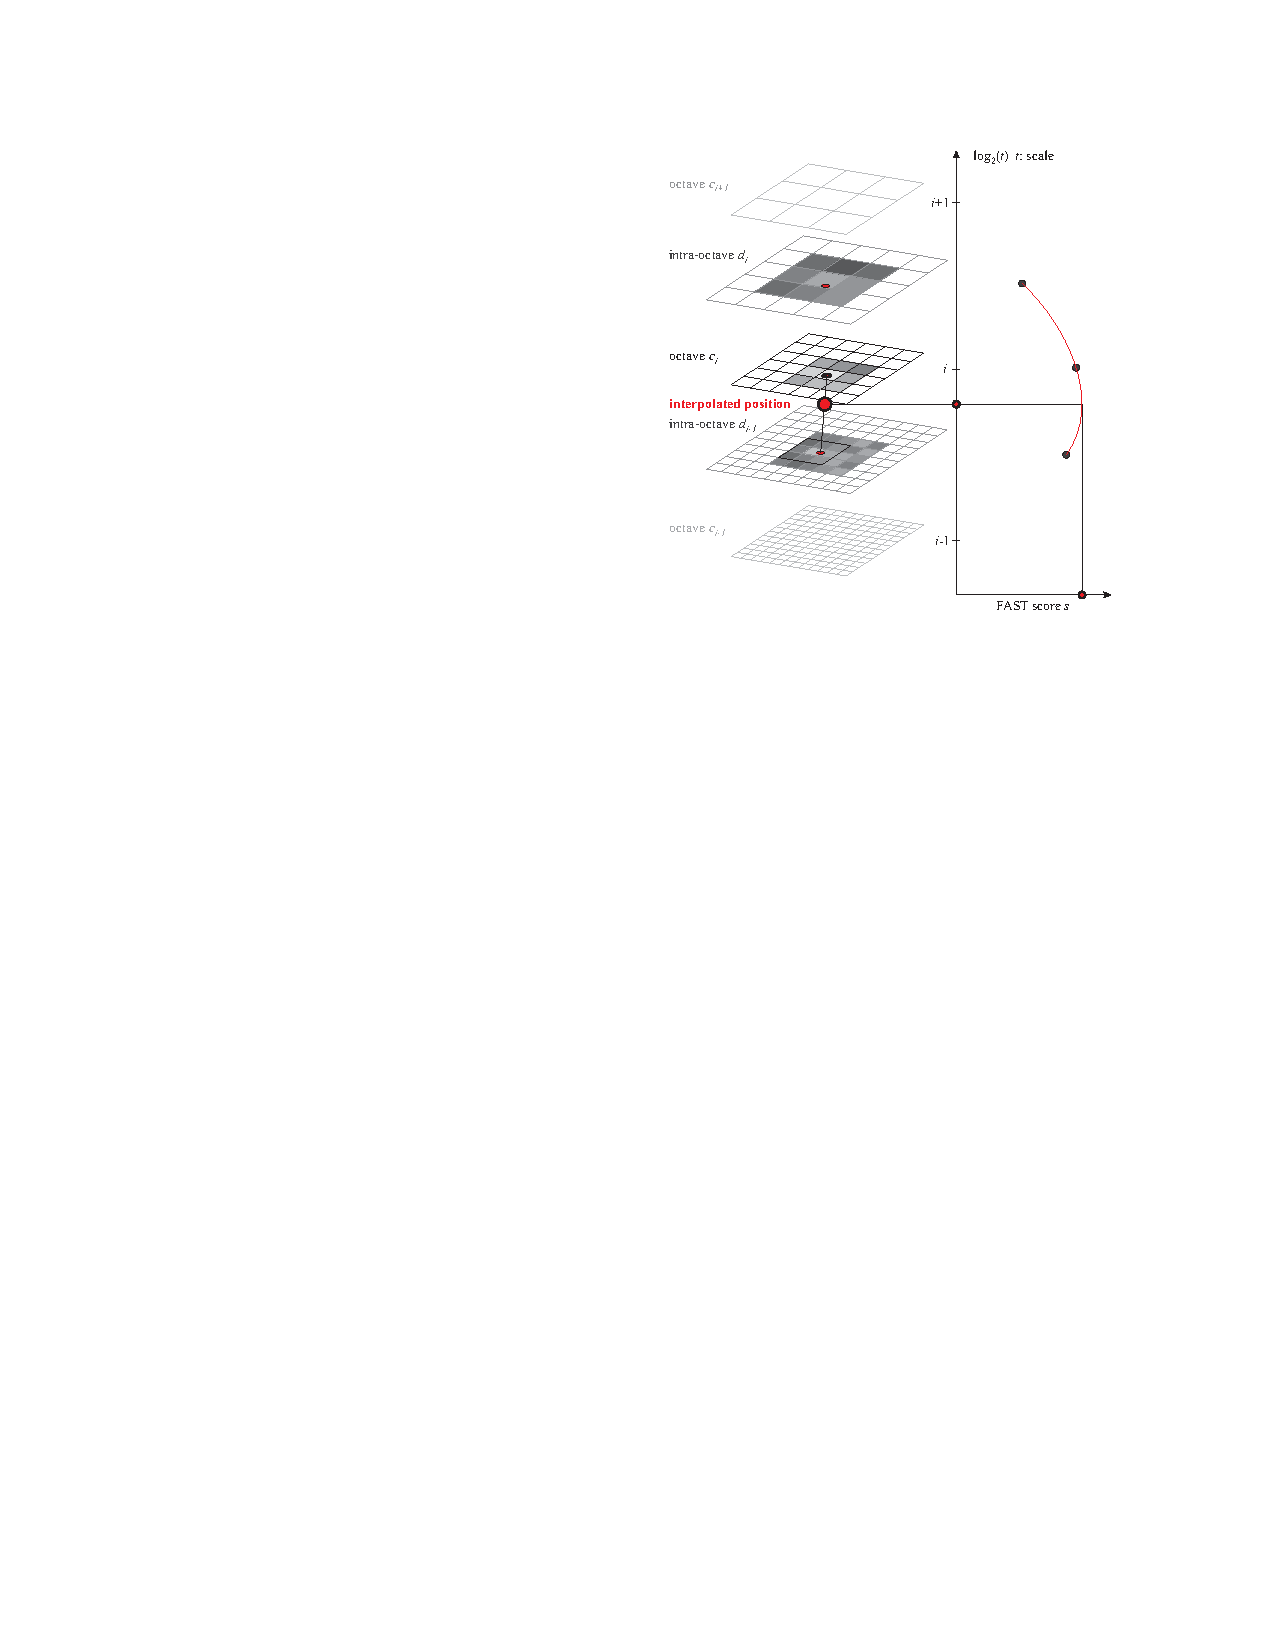
\includegraphics[width=0.8\textwidth]{../Drawings/methods/BRISKScaleSpace.pdf}
    \caption{Sub-pixel refinement and scale refinement is performed by interpolating a 1D parabola along three separate scales}
    \label{fig:1dparabola}
\end{figure}

This procedure is performed on all detected maxima and this produces a set of interest points with sub-pixel refined image locations as well as true scale values. The descriptors for these interest points are subsequently determined.

\subsubsection{Descriptor}
\label{sec:briskDescribe}
One of the important aspects of the BRISK descriptor is that it uses a pre-determined pattern to sample the neighborhood surrounding each detected interest point $k$. Equally spaced samples, $p_i$ are chosen which are placed on concentric circles centered on the interest point. This is shown in \figref{fig:samplingPattern} \citep{Leutenegger2011}. Aliasing can occur and in order to prevent this problem, Gaussian smoothing is applied to each sampled point on the concentric circles with standard deviation $\sigma_i$ proportional to the difference between the sampled points on the circle. \\

\begin{figure}[h!] 
  \centering
    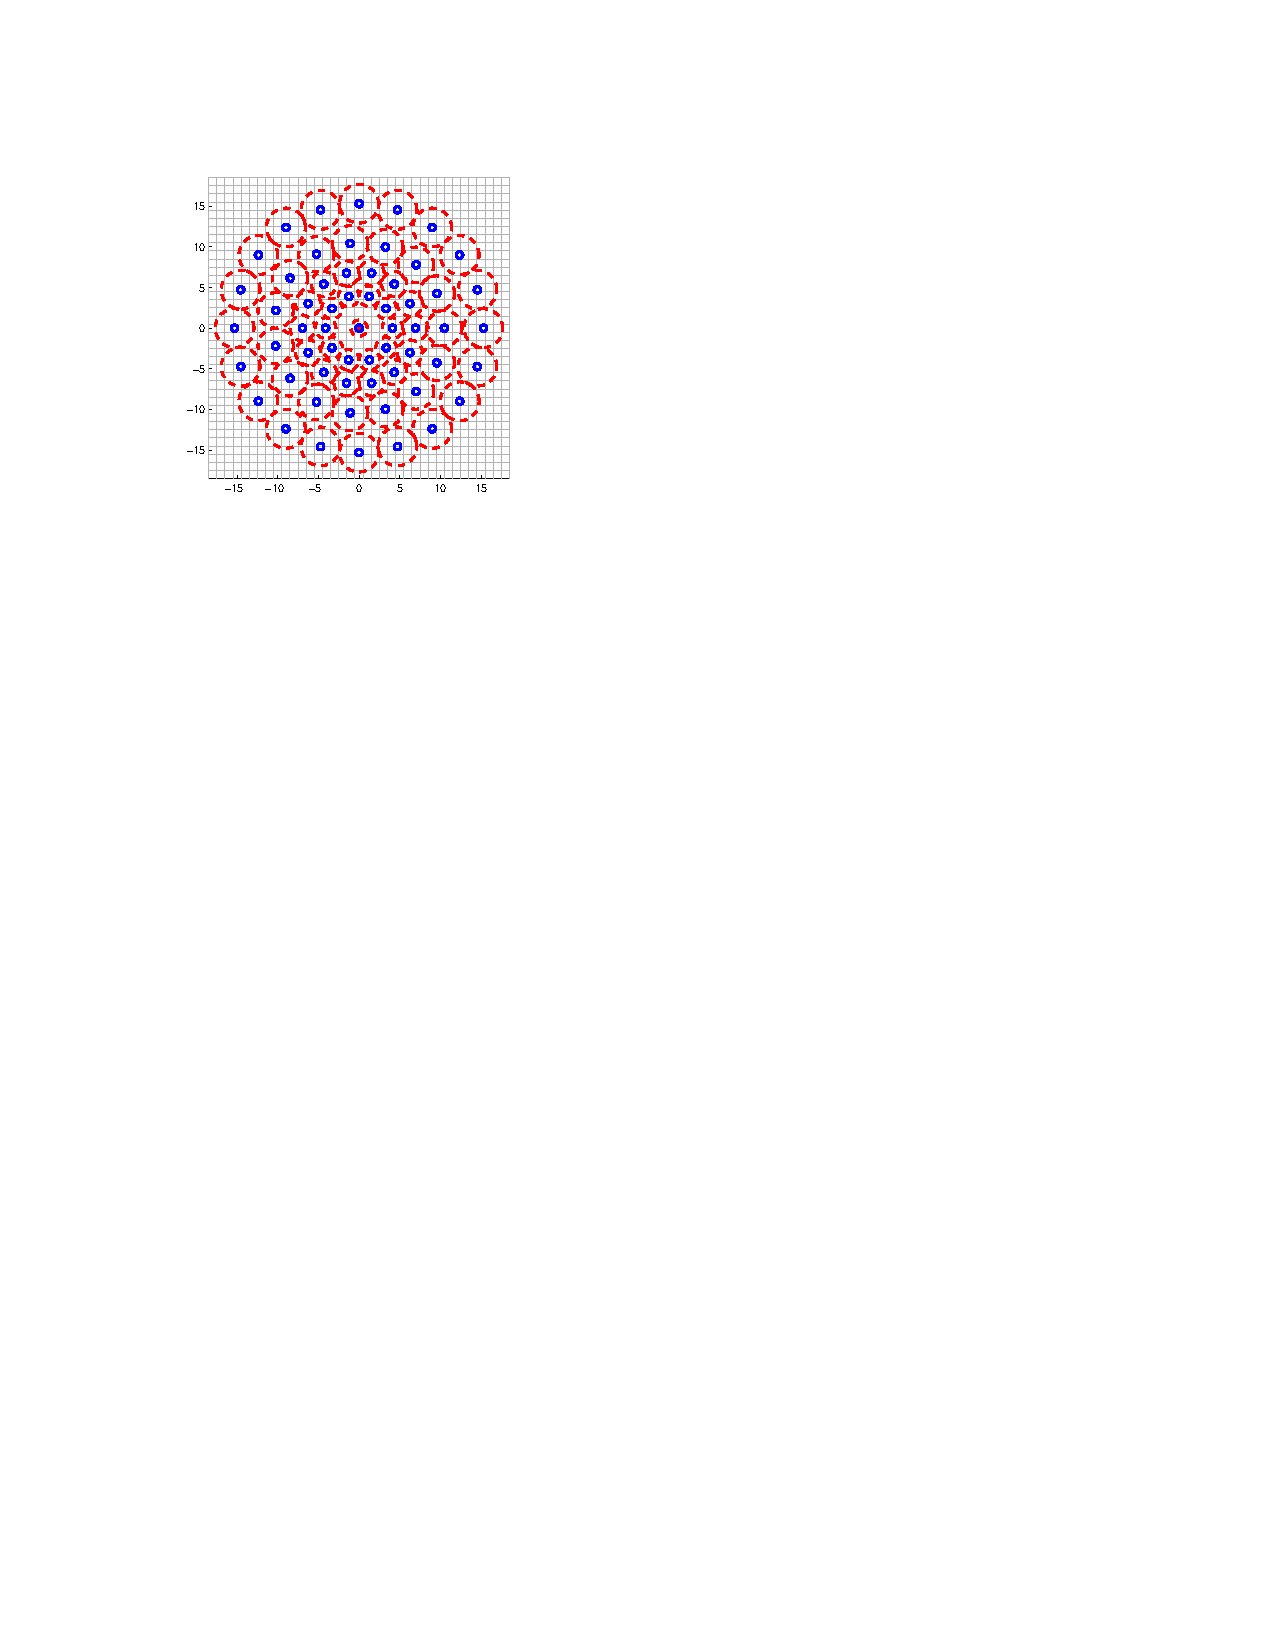
\includegraphics[width=0.8\textwidth]{../Drawings/methods/BRISK_Sampling_Pattern.pdf}
    \caption{The sampling pattern for an interest point. Each blue circle represents a sample and the red circle size is proportional to the amount of smoothing performed on each respective sample}
    \label{fig:samplingPattern}
\end{figure}

The next step is to position and scale the pattern according to the interest points that have been detected. The first step in the procedure is to calculate the gradient between each of the points $(p_i, p_j)$ in the pattern. This gradient is calculated as shown in \eqnref{eqn:gradient}.\\

\begin{equation}
m(p_i, p_j) = (p_j - p_i) \frac{I(p_j, \sigma_j) - I(p_i, \sigma_i)}{||p_j - p_i||^2}
\label{eqn:gradient}
\end{equation}

Following this, the euclidean distance between all possible pairings of the sample points are computed to generate long and short pairs, $L$ and $S$ respectively. The pairings are defined as shown in \eqnref{eqn:pairings}. The thresholds $ \delta_{max},  \delta_{min}$ are chosen as $9.75h$ and $13.67h$ where $h$ is the scale of the interest point $k$. \\   


\begin{eqnarray}
S &=& ((p_i, p_j) \mid ||p_j - p_i|| < \delta_{max})\\
L &=& ((p_i, p_j) \mid ||p_j - p_i|| > \delta_{min})
\label{eqn:pairings}
\end{eqnarray} 

The overall pattern direction for the interest point is determined by computing the overall gradient of all the long pairings $L$ as shown in \eqnref{eqn:longGradients}. Long pairings are used instead of short pairings as it was found that short pairing gradients tend to cancel each other out \citep{Leutenegger2011}. \\

\begin{equation}
\textbf{M} = (m_x, m_y) = \frac{1}{L} \sum_{((p_i, p_j) \epsilon L)} m(p_i,p_j)
\label{eqn:longGradients}
\end{equation}

This gradient is then used to find the angle with which to rotate the sampling pattern around the interest point in order to achive rotation invariance. The angle is computed as shown in \eqnref{eqn:angle}. \\

\begin{equation}
\alpha = atan(\frac{m_y}{m_x})
\label{eqn:angle}
\end{equation}

Once the pattern has been rotated, the descriptor vector is computed. This vector is $512$ bits long and is formed using intensity comparisons between the rotated short distance pairings $S$. Therefore, for each short-distance pairing, a brightness comparison test as shown in \eqnref{eqn:brightness} is performed to yield the descriptor entry $d_k$, $k = 1,2,3...512$.\\

\begin{equation}
d_k = \left\{ \begin{array}{rl}
1 &\mbox{$I(p_j^{\alpha}, \sigma_j) > I(p_i^{\alpha}, \sigma_i)$,} \\
0 &\mbox{Otherwise}
\end{array} \right.
\label{eqn:brightness}
\end{equation}

This produces the rotation and scale invariant descriptor vector.\\